\documentclass[10pt]{article}

\usepackage[latin1]{inputenc}
\usepackage{amsmath, amssymb, amsfonts, amsthm}
\usepackage{upgreek}
\usepackage{amsthm}
\usepackage{fullpage}
\usepackage{graphicx}
\usepackage{cancel}
\usepackage{subfigure}
\usepackage{mathrsfs}
\usepackage{outlines}
\usepackage[font={sf,it}, labelfont={sf,bf}, labelsep=space, belowskip=5pt]{caption}
\usepackage{hyperref}
% \usepackage{minted}
\usepackage{titling}
\usepackage{xifthen}
\usepackage{color}

\usepackage{fancyhdr}
\usepackage[title]{appendix}
\usepackage{float}

\usepackage{import}

\usepackage{bm}

\newcommand{\documenttitle}{Elastic Rod Scissor Linkages}

\DeclareMathOperator{\tr}{tr}
\DeclareMathOperator{\sgn}{sgn}
\DeclareMathOperator{\sinc}{sinc}
\DeclareMathOperator{\rref}{rref}
\DeclareMathOperator{\cof}{cof}
\DeclareMathOperator*{\sym}{sym}

\DeclareMathOperator{\diag}{diag}
\DeclareMathOperator*{\argmax}{argmax}
\DeclareMathOperator*{\argmin}{argmin}
\newcommand{\defeq}{\vcentcolon=}
\renewcommand{\Re}{\operatorname{Re}} \renewcommand{\Im}{\operatorname{Im}}
\allowdisplaybreaks

\pagestyle{fancy}
\headheight 24pt
\headsep    12pt
\lhead{\documenttitle}
\rhead{\today}
\fancyfoot[C]{} % hide the default page number at the bottom
\lfoot{}
\rfoot{\thepage}
\renewcommand{\headrulewidth}{0.4pt}
\renewcommand\footrulewidth{0.4pt}
\providecommand{\abs}[1]{\lvert#1\rvert}
\providecommand{\norm}[1]{\lVert#1\rVert}
\providecommand{\normlr}[1]{\left\lVert#1\right\rVert}
\providecommand{\dx}{\, \mathrm{d}x}
% \providecommand{\vint}[2]{\int_{#1} \! #2 \, \mathrm{d}x}
% \providecommand{\sint}[2]{\int_{\partial #1} \! #2 \, \mathrm{d}A}
\renewcommand{\div}{\nabla \cdot}
\providecommand{\cross}{\times}
\providecommand{\curl}{\nabla \cross}
\providecommand{\grad}{\nabla}
\providecommand{\laplacian}{\bigtriangleup}
\providecommand{\shape}{\Omega}
\providecommand{\mesh}{\mathcal{M}}
\providecommand{\boundary}{\partial \shape}
\providecommand{\vint}[3][\x]{\int_{#2} \! #3 \, \mathrm{d}#1}
\providecommand{\sint}[3][\x]{\int_{#2} \! #3 \, \mathrm{d}A(#1)}
\providecommand{\lint}[3][\x]{\int_{#2} \! #3 \, \mathrm{d}s(#1)}
\providecommand{\pder}[2]{\frac{\partial #1}{\partial #2}}
\providecommand{\spder}[3]{\frac{\partial^2 #1}{\partial #2 \partial #3}}
\providecommand{\tder}[2]{\frac{\mathrm{d} #1}{\mathrm{d} #2}}
\providecommand{\evalat}[2]{\left.#1\right|_{#2}}
\renewcommand{\vec}[1]{{\bf #1}}

\providecommand{\tderatzero}[2]{\left.\frac{\mathrm{d} #1}{\mathrm{d} #2}\right|_{#2 = 0}}

\newcommand{\TODO}[1]{\textbf{****** {\bf{[#1]}} ******}}

\usepackage{prettyref}
\newrefformat{sec}{Section~\ref{#1}}
\newrefformat{tbl}{Table~\ref{#1}}
\newrefformat{fig}{Figure~\ref{#1}}
\newrefformat{chp}{Chapter~\ref{#1}}
\newrefformat{eqn}{\eqref{#1}}
\newrefformat{set}{\eqref{#1}}
\newrefformat{alg}{Algorithm~\ref{#1}}
\newrefformat{apx}{Appendix~\ref{#1}}
\newrefformat{prop}{Proposition~\ref{#1}}
\newcommand\pr[1]{\prettyref{#1}}

\def\normal{{\bf n}}
\def\n{\normal}
\def\a{\vec{a}}
\def\b{\vec{b}}
\def\d{\vec{d}}
\def\t{\vec{t}}
\def\x{\vec{x}}
\def\X{\vec{X}}
\def\y{\vec{y}}
\def\z{\vec{z}}
\def\u{\vec{u}}
\def\f{\vec{f}}
\def\w{\boldsymbol{\omega}}
\def\p{\vec{p}}
\def\r{\vec{r}}
\def\v{\vec{v}}
\def\e{\vec{e}}
\def\thvec{{\bm \theta}}
\def\ue{\vec{u}^\e}
\def\fu{\pder{\f}{u}}
\def\fv{\pder{\f}{v}}
\def\strain{\varepsilon}
\def\stress{\sigma}
\def\kb{\kappa \b}
\def\kbi{(\kappa \b)_i}
\def\k{\kappa}
\def\R{\, \mathbb{R}}
\def\L{\, \mathcal{L}}
\def\segment{s}
\def\joint{\jmath}

\providecommand\ts[1]{\widehat{\vec{t}^{#1}}}
\providecommand\ds[2]{\widehat{\vec{d}^{#1}_{#2}}}
\providecommand\rd[2]{\underline{\vec{d}^{#1}_{#2}}}
\providecommand\rds[2]{\widehat{\underline{\vec{d}^{#1}_{#2}}}}
\providecommand{\PXport}[1]{P_{\ts{#1}}^{\t^{#1}}}

\providecommand\tsA{\hat{\vec{t}}_A}
\providecommand\tsB{\hat{\vec{t}}_B}
\providecommand\ns{\hat{\vec{n}}}

\providecommand{\compose}{\circ}
\providecommand{\surface}{\Gamma}
\providecommand{\surfacegrad}{\nabla_\surface}
\providecommand{\surfacediv}{\surfacegrad \cdot}
\providecommand{\surfacelaplacian}{\laplacian_\surface}

\providecommand{\epssurface}{{\Gamma_\epsilon}}
\providecommand{\epssurfacegrad}{\nabla_\epssurface}
\providecommand{\epssurfacediv}{\epssurfacegrad \cdot}
\providecommand{\epsnormal}{\normal_\epsilon}
\providecommand{\epsnormalmat}{\tilde{\normal}_\epsilon}
\providecommand{\epsphi}{\phi_\epsilon}
\providecommand{\normalmatder}{\dot{\normal}}
\providecommand{\shapefunc}{{\bm \phi}}

\def\vt{\vec{v}_t}
\def\k{\kappa}

\newcommand*{\rom}[1]{\expandafter\@slowromancap\romannumeral #1@}
\newcommand{\RN}[1]{\textup{\uppercase\expandafter{\romannumeral#1}}}

\newtheorem{lemma}{Lemma}
\newtheorem{proposition}{Proposition}
\newtheorem{corollary}{Corollary}

\makeatletter
\usepackage{mathtools}
\newcases{mycases}{\quad}{%
  \hfil$\m@th\displaystyle{##}$}{$\m@th\displaystyle{##}$\hfil}{\lbrace}{.}
\makeatother

\setlength{\droptitle}{-50pt}
\title{\documenttitle}
\author{Julian Panetta}

% BEGIN DOCUMENT
\begin{document}
\maketitle

We describe how to model the static equilibria of linkages formed by elastic rods connecting at scissor joints.
Our linkage model builds on the popular discrete elastic rods model of \cite{Bergou2010}.

\section{Rod Linkage Graph}
\begin{figure}[h]
    \centering
    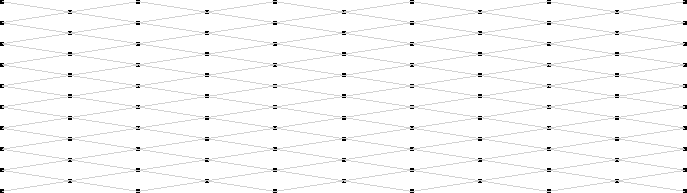
\includegraphics[width=.5\textwidth]{images/linkage_screenshot.png}
    \caption{An example graph defining a rod linkage.}
    \label{fig:linkage_example}
\end{figure}
The linkage's initial configuration is defined by an embedded graph (i.e., line
mesh) with vertices and edges ($V$, $E$).
Each edge of this graph is referred to as a rod \emph{segment}, and generally
these segments continue across the vertices to form a complete rod as shown in
\pr{fig:linkage_example}.

Each graph
vertex represents either a scissor joint or a rod's free end. Vertex valences can be
one (free end), two (two rod ends pinned together), three (one rod's
end pinned to another's interior), or four (two rods pinned together in their
interior). We prohibit valences above four. \pr{fig:linkage_example} shows
examples of each of these valences.

Each rod segment is modeled as a \emph{distinct} discrete elastic rod with
$n_s$ subdivisions. We will see how to properly couple the segments making up a
full rod so that they behave just like one large elastic rod. We label the
$n^\text{th}$ segment $\segment_n$ for $n \in \{0\dots|E| - 1\}$ and the joints
$\joint_i$ for $i \in \{0\dots|J| - 1\}$, where $J \subset V$ is the set of
vertices of valence $2\text{--}4$.

\section{Rod and Joint Representation}
Recall that a discrete elastic rod's configuration is defined by its centerline positions
and its material frame angles (expressed relative to the rod's hidden reference
frame state). The material frame is used to express the orientation/twist of
the rod's cross sections, which is particularly important for flat, anisotropic
rods.

The rod segments meeting at a joint can be partitioned into two sets, one for
each full rod passing through the joint. This partitioning is done by determining
which segments connect to form the straightest path across the vertex in the
rest configuration. We need to glue together the segments making up a rod and allow
the two incident rods pivot around the vertex. We accomplish this gluing by
having the joint impose the same terminal edge vector for the segments
connecting to form a single rod. Also, the joint constrains the orientation of
all incident segments' centerlines: the second material axis $\d_2$ must be
normal to the plane spanned by both incident centerline edges. See
\pr{fig:joint_example} for an example joint configuration.

\begin{figure}[h]
    \centering
    \def\svgwidth{.5\textwidth}
    \import{images/}{joint_geometry.pdf_tex}
    \caption{The geometry of rod scissor linkages. Here we visualize the
    linkage graph for a single scissor linkage (comprising four rod segments)
    and the corresponding rod geometry. The joint parameters determine the edge
    vectors and material frame for the terminal edges of all incident rod
    segments.} \label{fig:joint_example}
\end{figure}

\section{Linkage Degrees of Freedom}
Our rod linkage model incorporates the constraints imposed by the joints by
constructing a reduced set of variables that parametrize all
admissible rod configurations. These reduced variables consist of (in order):
\begin{itemize}
    \item For each rod segment $\segment \in E$ :
    \begin{itemize}
        \item Centerline positions for all interior and free-end nodes of $s$.
            The $x$, $y$, and $z$ coordinates of the first interior/free node
            come first, followed by the coordinates for all subsequent
            nodes.
        \item Material frame angles $\theta$ for all interior and free-end edges of
              $\segment$.
    \end{itemize}
    \item Parameters for each joint $\joint \in J$: position and edge vectors $\p, \e_A, \e_B
        \in \R^3$ flattened in $x$, $y$, $z$ order.
\end{itemize}
We implement two types of joints, constrained and unconstrained. An unconstrained
joint is specified by two vectors, indicating the direction and length of the two
centerline edges pivoting around the vertex. A constrained joint has a fixed
direction for both of these centerline edges, and only their lengths are
variables. In both cases, the joint parameters completely determine the
degrees of freedom (centerline positions and $\theta$s) for the terminal edges
of all rod segments incident the joint. See \pr{fig:joint_example} for a visualization of how
the joint's degrees of freedom $\e_A$ and $\e_B$ determine the geometry of the
incident rod edges. The material axis angle $\theta$ for a given incident rod
segment edge is determined from that edge's current reference frame
${(\underline{\d_1}, \underline{\d_2})}$ and the relationship:
$$
\d_2 = \n \defeq \frac{\e_A \cross \e_B}{\norm{\e_A \cross \e_B}}.
$$

\section{Elastic Energy, Gradients, and Hessians}
Our model's joints store no energy, so the elastic energy of the full
linkage is computed by summing the energy from each rod segment. We can then
compute derivatives of this energy with respect to our degrees of
freedom by assembling the (transformed) derivatives of the discrete
elastic rod model.

\subsection{Gradients}
Since $\e_A$ and $\e_B$ directly determine the segments' incident edge vectors,
it's straightforward to compute by chain rule the gradient contribution due to
the changing centerline. The only challenging part is computing with the
contributions from the changing material frame angles induced by the constraint
$\d_2 = \n$. For this, we use chain rule and the relationship:
\begin{align*}
    \left(\pder{\theta^j}{\e_A}\right)^T &= -\d^j_1 \cdot \pder{\n}{\e_A} + \underline{\d^j_1} \cdot \pder{\PXport{j} \underline{\ds{j}{2}}}{\e_A} \\
    \left(\pder{\theta^j}{\e_B}\right)^T &= -\d^j_1 \cdot \pder{\n}{\e_B} + \underline{\d^j_1} \cdot \pder{\PXport{j} \underline{\ds{j}{2}}}{\e_B}.
\end{align*}
The first terms capture the rotation of $\d_2 = \bf{n}$, and the second subtract off the rotation of the reference frame due to parallel transport.
Note that, for a given terminal edge ``j,''  only one of the second terms will
appear, depending on whether the edge is part of rod $A$ or $B$.

We already obtained an expression for the parallel transport term when deriving the finite
transport twist energy gradient for discrete elastic rods:
$$
\underline{\d^j_1} \cdot \pder{\PXport{j} \rds{j}{2}}{\e_j}
    =
        \frac{I - \t^j \otimes \t^j}{\norm{\e^j}}
        \bigg(
            \frac{
                \big(\rds{j}{1} \cdot \t^{j}\big)\big(\rd{j}{1} \cross \ts{j}\big) + \big(\rd{j}{2} \cdot \ts{j}\big) \rds{j}{1}
            }{1 + \ts{j} \cdot \t^{j}}
            - \frac{\big(\rds{j}{1} \cdot \t^{j}\big)\big(\rd{j}{2} \cdot \ts{j} \big) }{(1 + \ts{j} \cdot \t^{j})^2} \ts{j}
            + \rds{j}{1} \cross \rd{j}{1}
        \bigg).
$$
We compute the normal rotation term as follows:
\begin{align*}
    -\d^j_1 \cdot \pder{\n}{\e_A} &= -\d^j_1 \cdot \frac{(I - \cancelto{\perp}{\n} \otimes \n) [\e_B]_\cross^T}{\norm{\e_A \cross \e_B}}
        = \frac{\left(\d^j_1 \cross \e_B\right)^T}{\norm{\e_A \cross \e_B}}
        = -\frac{\t^j \cdot \e_B}{\norm{\e_A \cross \e_B}}\n^T.
\\
    -\d^j_1 \cdot \pder{\n}{\e_B} &= -\d^j_1 \cdot \frac{(I - \cancelto{\perp}{\n} \otimes \n) [\e_A]_\cross}{\norm{\e_A \cross \e_B}}
        = \frac{\left(\e_A \cross \d^j_1\right)^T}{\norm{\e_A \cross \e_B}}
        = \, \, \, \, \frac{\t^j \cdot \e_A}{\norm{\e_A \cross \e_B}}\n^T.
\end{align*}
Therefore:
\begin{align*}
    \pder{\theta^j}{\e_A} &=
        -\frac{\t^j \cdot \e_B}{\norm{\e_A \cross \e_B}}\n +
        s_{jA} \frac{(I - \t_A \otimes \t_A)}{\norm{\e_A}} \left(
                \frac{
                    \big(\rds{j}{1} \cdot \t^{j}\big)\big(\rd{j}{1} \cross \ts{j}\big) + \big(\rd{j}{2} \cdot \ts{j}\big) \rds{j}{1}
                }{1 + \ts{j} \cdot \t^{j}}
                - \frac{\big(\rds{j}{1} \cdot \t^{j}\big)\big(\rd{j}{2} \cdot \ts{j} \big) }{(1 + \ts{j} \cdot \t^{j})^2} \ts{j}
                + \rds{j}{1} \cross \rd{j}{1}
        \right)
    \\
    \pder{\theta^j}{\e_B} &=
        \, \, \, \, \frac{\t^j \cdot \e_A}{\norm{\e_A \cross \e_B}}\n +
        s_{jB} \frac{(I - \t_B \otimes \t_B)}{\norm{\e_B}} \left(
                \frac{
                    \big(\rds{j}{1} \cdot \t^{j}\big)\big(\rd{j}{1} \cross \ts{j}\big) + \big(\rd{j}{2} \cdot \ts{j}\big) \rds{j}{1}
                }{1 + \ts{j} \cdot \t^{j}}
                - \frac{\big(\rds{j}{1} \cdot \t^{j}\big)\big(\rd{j}{2} \cdot \ts{j} \big) }{(1 + \ts{j} \cdot \t^{j})^2} \ts{j}
                + \rds{j}{1} \cross \rd{j}{1}
        \right),
\end{align*}
where
$$
s_{jX} =
\begin{mycases}
    0 & \text{if terminal edge $j$ isn't part of rod $X$}, \\
    1 & \text{if terminal edge $j$'s orientation agrees with joint edge vector $\e_X$, or} \\
    -1 &\text{if terminal edge $j$'s orientation disagrees with joint edge vector $\e_X$}.
\end{mycases}
$$

\subsection{Hessian}

Next, we compute the Hessian with respect to our reduced variables. We express the elastic energy as
$$
E(\v(\r)),
$$
where vectors $\v$ and $\r$ collect the linkage's full and reduced variables.
So $\v$ contain the centerline positions $\x$ and material frame angles
$\theta$ for all rod segments, and $\r$ contains the unconstrained centerline
positions and material frame angles as well as the joint parameters $\e_A$ and
$\e_B$ controlling the constrained segment variables.
The gradient and Hessian with respect to the reduced variables can now be computed using the chain rule:
$$
\pder{E}{r_i} = \pder{E}{v_k}(\v(\r)) \pder{v_k}{r_i}
$$
$$
\spder{E}{r_i}{r_j} =
\pder{v_k}{r_i} \spder{E}{v_k}{v_l} \pder{v_l}{r_j}
+
\pder{E}{v_k} \spder{v_k}{r_i}{r_j}.
$$
For all the unconstrained variables (segments' interior/free end quantities),
$\pder{v_k}{r_i}$ is essentially just a Kronecker delta (1 if reduced variable
$r_i$ corresponds to unconstrained variable $v_k$, 0 otherwise). The Hessians
of these $v_k$ are zero, and all that remains is the first term, which is just
a permutation of the sub-block of the unreduced Hessian corresponding to the
unconstrained variables. We implement this by simply re-indexing the sparse
matrix entries.

The terminal edge centerline positions are simply linear functions of the
joint parameters, so again the term involving the Hessian of $v_k$ vanishes.
Note: these rows/columns of $\pder{v_k}{r_i}$ have multiple nonzero entries.
Finally, the terminal edge material frame angles are nonlinear functions of the
joint parameters, so for these we do need to compute second Hessian term:
$$
\pder{E}{\theta^j} \spder{\theta^j}{\e_X}{\e_Y}.
$$
Like when we derived the elastic rod energy Hessians, we simplify our
expressions by evaluating the Hessian only at the configuration from which the
source reference frame was set.
\begin{align*}
\spder{\theta^j}{\e_A}{\e_A} &=
        -\frac{\n}{\norm{\e_A \cross \e_B}} \otimes 
            \underbrace{\left(\frac{I - \t_A \otimes \t_A}{\norm{\e_A}} \e_B \right)s_{jA}}_{\norm{\e_A \cross \e_B} \frac{\n \cross \t^j}{\norm{\e_A}^2} \delta_{jA}}
        +\frac{\t^j \cdot \e_B}{\norm{\e_A \cross \e_B}^2}\left(I - 2 \n \otimes \n \right) [\e_B]_\cross
        + s_{jA}^2 \frac{[\t^j]_\cross}{2 \norm{\e^j}^2}
    \\
    &=
        -\frac{\n \otimes (\n \cross \t^j)}{\norm{\e_A}^2} \delta_{jA}
        +\frac{\t^j \cdot \e_B}{\norm{\e_A \cross \e_B}^2}\left(I - 2 \n \otimes \n \right) [\e_B]_\cross
        + \delta_{jA} \frac{[\t^j]_\cross}{2 \norm{\e_A}^2}
    \\
    &=
        -\frac{\d_2^j \otimes \d_1^j + \d_1^j \otimes \d_2^j}{2 \norm{\e_A}^2} \delta_{jA}
        +\frac{\t^j \cdot \e_B}{\norm{\e_A \cross \e_B}^2}\left(I - 2 \d_2^j \otimes \d_2^j \right) [\e_B]_\cross,
\end{align*}
where $\delta_{jX} \defeq s_{jX}^2$ is 1 if joint parameter $\e_A$ controls terminal edge $j$ and 0 otherwise.

Note, the last step of this derivation can be interpreted either as symmetrizing this Hessian block or plugging in the identity
${[\t^j]_\cross = \d^j_2 \otimes \d^j_1 - \d^j_1 \otimes \d^j_2}$. Also, we used the fact $s_{jA} \t_A = \t^j$.
Likewise, we find:
\begin{align*}
    \spder{\theta^j}{\e_B}{\e_B} &=
        \frac{\n}{\norm{\e_A \cross \e_B}} \otimes 
            \underbrace{\left(\frac{I - \t_B \otimes \t_B}{\norm{\e_B}} \e_A \right)s_{jB}}_{-\norm{\e_A \cross \e_B} \frac{\n \cross \t^j}{\norm{\e_B}^2} \delta_{jB}}
        +\frac{\t^j \cdot \e_A}{\norm{\e_A \cross \e_B}^2}\left(I - 2 \n \otimes \n \right) [\e_A]_\cross
        + s_{jB}^2 \frac{[\t^j]_\cross}{2 \norm{\e^j}^2}
    \\
    &=
        -\frac{\d_2^j \otimes \d_1^j + \d_1^j \otimes \d_2^j}{2 \norm{\e_B}^2} \delta_{jB}
        +\frac{\t^j \cdot \e_A}{\norm{\e_A \cross \e_B}^2}\left(I - 2 \d_2^j \otimes \d_2^j \right) [\e_A]_\cross.
\end{align*}
Finally, we compute the cross terms:
\begin{align*}
    \left(\spder{\theta^j}{\e_B}{\e_A}\right)^T =
    \spder{\theta^j}{\e_A}{\e_B} &=
    -\frac{\n \otimes \t^j}{\norm{\e_A \cross \e_B}}
    - \frac{(\t^j \cdot \e_B)(I - 2 \n \otimes \n) [\e_A]_\cross}{\norm{\e_A \cross \e_B}^2}.
\end{align*}

\section{Rotation-based Joint Representation}
\begin{figure}[h]
    \centering
    \def\svgwidth{.5\textwidth}
    \import{images/}{new_joint_parametrization.pdf_tex}
\end{figure}
The parameterization used above for the joints, though simplifying the
dependence of rod state on the joint parameters, has several drawbacks. First,
it will become ill-conditioned/degenerate as $\e_A$ and $\e_B$ become nearly parallel.
Second, the joint's orientation is coupled with the opening angle, so it's no possible
to pin down rigid motion by constraining a joint without also fixing the opening angle.
Third, the opening angle is not an explicit parameter in the system, making it
difficult to formulate more global deployment actuations (writing
energies/constraints in terms of the angles at all joints).

We therefore opt to parametrize each joint by a position, $\p$, a
global rotation/frame (represented as an angle-scaled axis vector, $\w$),
an opening angle $\alpha$ between rods $A$ and $B$, and the deformed length of
the edge vectors. Since a joint can be constrained by fixing its $\p$, $\w$, and
$\alpha$ variables, we no longer need to use a separate parametrization
for ``constrained joints'' as described above; we can impose joint constraints
just by fixing variables in the optimization.

The joint's incident edge vectors $\e_A$ and $\e_B$ and joint normal are then:
$$
\e_A = R(\w) \tsA l_A, \quad
\e_B = R(\w) \underbrace{\Big(\tsA \cos(\alpha) + (\ns \cross \tsA) \sin(\alpha)\Big)}_{\defeq \tsB(\alpha)} l_B, \quad
\n = R(\w) \ns,
$$
where $\tsA$ and $\ns$ are the ``source''/initial rod $A$ tangent and joint normal vectors
(also stored in each joint).
These can be interpreted as defining a reference rotation matrix
$R_0 \defeq \left(\begin{array}{c|c|c} \tsA & \ns \cross \tsA & \ns \end{array}\right)$,
so that $\w$ is a vector in the tangent space of $SO(3)$ at $R_0$ (see the
documentation in the \texttt{RotationOptimization} repository).

As before, the joint's normal $\n$ determines the material axis $\d_2$ for all
incident rod edges (controlling their $\theta$ parameters). The edge vectors $\e_A$ and $\e_B$
control the centerline positions of the incident rod edges, placing them at,
e.g., $\p \pm \frac{1}{2} \e_A$.
The \emph{nonzero} blocks of the gradient of these edge vectors and $\theta^j$ are:
\begin{align*}
    \pder{\e_A}{\w} &= \pder{(R(\w) \tsA)}{\w}l_A, \quad
    \pder{\e_A}{l_A}= R(\w) \tsA, \\
    \pder{\e_B}{\w} &= \pder{\left(R(\w) \tsB(\alpha) \right)}{\w} l_B, \quad
    \pder{\e_B}{\alpha} = R(\w) \underbrace{\Big(-\tsA \sin(\alpha) + (\ns \cross \tsA) \cos(\alpha) \Big)}_{\defeq \tsB^\perp(\alpha)} l_B, \quad
    \pder{\e_B}{l_B} = R(\w) \tsB(\alpha) \\
%   \pder{\e_B}{\alpha} &= \pder{\e_A}{l_A} = 0 \\
    \left(\pder{\theta^j}{\w}\right)^T &= -\d^j_1 \cdot \pder{\n}{\w}
    + \underline{\d^j_1} \cdot \left(s_{jA} \pder{P_{\ts{j}}^{\t_A} \underline{\ds{j}{2}}}{\t_A} \pder{\t_A}{\w} + s_{jB} \pder{P_{\ts{j}}^{\t_B} \underline{\ds{j}{2}}}{\t_B} \pder{\t_B}{\w} \right),
\quad
    \pder{\theta^j}{\alpha} = s_{jB} \underline{\d^j_1} \cdot \left(\pder{P_{\ts{j}}^{\t_B} \underline{\ds{j}{2}}}{\t_B} \pder{\t_B}{\alpha} \right),
\end{align*}
where the terms involving $\underline{\d^j_1}$ subtract off the rotation of the reference frame due to parallel transport.
Note that this parallel transport term vanishes if the source frame has been updated.
The terms here like $\pder{(R(\w) \tsA)}{\w}$ can be evaluated with the gradient-of-rotated-vector function
provided by \texttt{RotationOptimization}.
The Hessian blocks of the edge vectors are:
\begin{equation*}
\boxed{
\begin{aligned}
    \spder{\e_A}{\w}{\w} &= \spder{(R(\w) \tsA)}{\w}{\w} l_A, \quad
    \spder{\e_A}{\w}{l_A} = \pder{(R(\w) \tsA)}{\w},
\\
    \spder{\e_B}{\w}{\w} &= \spder{\left(R(\w) \tsB(\alpha) \right)}{\w}{\w} l_B, \quad
    \spder{\e_B}{\w}{l_B} = \pder{\left(R(\w) \tsB(\alpha) \right)}{\w}, \quad
    \spder{\e_B}{\w}{\alpha} = \pder{\left(R(\w) \tsB^\perp(\alpha) \right)}{\w} l_B,
\\
    \spder{\e_B}{l_B}{\alpha} &= R(\w) \tsB^\perp(\alpha), \quad
    \spder{\e_B}{\alpha}{\alpha} = -R(\w) \tsB(\alpha) l_B = -\e_B
\end{aligned}
}
\end{equation*}

To simplify the Hessian of $\theta^j$, we assume that the source frame has been updated
(i.e., we evaluate at $\t^j = \ts{j}$). Recall
the derivative
with respect to the edge tangent of (minus) the reference frame rotation:
$$
\left.\pder{}{\t^j}\right|_{\t^j = \ts{j}} \left[\underline{\d^j_1} \cdot \left(\pder{P_{\ts{j}}^{\t^j} \underline{\ds{j}{2}}}{\t^j} \right)\right]
= (\underline{\d^j_2} \otimes -\t^j) \cdot (-\t^j \otimes \underline{\d^j_1}) + \d^j_1 \cdot \left.\spder{P_{\ts{j}}^{\t^j}\underline{\ds{j}{2}}}{\t^j}{\t^j}\right|_{\t^j = \ts{j}}
= \underline{\d^j_2} \otimes \underline{\d^j_1} -
  \frac{\underline{\d^j_2} \otimes \underline{\d^j_1}  +
        \underline{\d^j_1} \otimes \underline{\d^j_2}}{2} = \frac{[\t^j]_\cross}{2}.
$$
\begin{equation*}
\boxed{
\begin{aligned}
    \spder{\theta^j}{\w}{\w} &= -\left(\pder{\n}{\w}\right)^T \pder{\d^j_1}{\w} - \d_1^j \cdot \spder{\n}{\w}{\w}
        + \delta_{jA} \left(\pder{\t_A}{\w}\right)^T \frac{[\t^j]_\cross}{2} \pder{\t_A}{\w}
        + \delta_{jB} \left(\pder{\t_B}{\w}\right)^T \frac{[\t^j]_\cross}{2} \pder{\t_B}{\w}
\\
    &= -\sym\left(\left(\pder{\n}{\w}\right)^T \pder{\d^j_1}{\w}\right) - \d_1^j \cdot \spder{\n}{\w}{\w},
\\
    \spder{\theta^j}{\alpha}{\w} &= 
        \delta_{jB} \left(\pder{\t_B}{\alpha}\right)^T \frac{[\t^j]_\cross}{2} \pder{\t_B}{\w} =
       -\frac{\delta_{jB}}{2} \left(\pder{\t_B}{\w}\right)^T \left(\t_B \cross \pder{\t_B}{\alpha}\right),
\\
    \spder{\theta^j}{\alpha}{\alpha} &= 
        \delta_{jB} \left(\pder{\t_B}{\alpha}\right)^T \frac{[\t^j]_\cross}{2} \pder{\t_B}{\alpha} = 0.
\end{aligned}
}
\end{equation*}

\bibliographystyle{plain}
\bibliography{DiscreteElasticRods}

\end{document}
